\documentclass{sig-alternate}
\usepackage{subfigure, graphicx, url}

\newcommand{\strong}[1] {\textbf{#1}}
\newcommand{\code}[1] {\texttt{#1}}

\begin{document}
\title{Text Sliding: Information Discovery with Intensely Integrated Text Analysis}
\numberofauthors{4}

\author{% 1st. author
\alignauthor Aditi Muralidharan\\
       \affaddr{Computer Science Division}\\
       \affaddr{UC Berkeley}\\
       \email{aditi@cs.berkeley.edu}
% 2nd. author
\alignauthor {Mart A.  Hearst}\\
       \affaddr{School of Information}\\
       \affaddr{UC Berkeley}\\
       \email{hearst@ischoo.berkeley.edu}
% 3rd. author
\alignauthor Christopher Fan\\
       \affaddr{English Department}\\
       \affaddr{UC Berkeley}\\
       \email{cfan@berkeley.edu}
}

\maketitle

\begin{abstract}

This paper describes WordSeer, a tool whose goal is to help scholars and analysts discover patterns and formulate and test hypotheses about the contents of  text collections, midway between what  humanities scholars call a traditional  ``close read'' and the new ``distant read'' or  ``culturomics" approach.  
To this end, we describe a text analysis and discovery tool that allows for highly flexible  ``slicing and dicing'' (hence  ``sliding'') across a text collection.  The tool allows users to view text from different angles by selecting subsets of data, viewing those as visualizations, moving laterally to view other subsets of data, slicing into another view, expanding the viewed data by relaxing constraints, and so on.  We illustrate the text sliding capabilities of the tool with two real-world case studies from the humanities and social sciences -- the practice of literacy education, and U.S. perceptions of China and Japan over the last 30 years -- showing how the tool has enabled scholars with no technical background to make new, important discoveries in these text collections.

\end{abstract}

\section{Introduction}
This paper describes a new tool for exploratory data analysis \cite{tukey1977exploratory} that attempts to provide frictionless access to text and its metadata.  Although many tools have been developed to analyze numerical and categorical data, language in its written form of text has special properties that makes it more difficult to analyze. Text has both linear and hierarchical structure, its meaning is ambiguous given its representation, it has tens of thousands or hundreds of thousands of features, and frequencies of words are usually distributed via a power law.  

Even a small fragment of text does not stand alone, but evokes, in the reader's mind, other texts containing the same words, phrases, or ideas. To an analyst trying to make sense of an idea, some associations may be deeply meaningful.  Transitions  and associations are central to the text analysis process, and people seeking knowledge from text are engaging in \emph{sensemaking}. They do not follow a straight path from data input to analysis output, but meander between analysis, interpretation, exploration and understanding on different sub-collections of data \cite{russell_cost_1993, pirolli_sensemaking_2005}. 

In this paper, we describe a text analysis tool called WordSeer that supports such transitions\footnote{WordSeer is a web application. This is version 3.0, which has notably more flexible interactions than older versions.}.  It allows highly flexible slicing and dicing, as well as frictionless transitions (hence ``sliding") between visual analyses, drill-downs, lateral explorations and overviews of slices in a text collection. Our tool uses computational linguistics, information retrieval and data visualization, and enables scholars with no technical background to conduct analyses yielding concrete, useful and otherwise inaccessible knowledge. 

We introduce the text sliding capabilities of WordSeer with a running example of a real-world case study with C.F.,  a scholar at UC Berkeley's English department. He studied how U.S. perceptions of China and Japan responded to China's rise over the last 30 years using a collection of 5,715  \emph{New York Times} editorials about China and Japan from 1980 to 2012. 

A video demonstrating WordSeer through examples from  this case study is available at \url{http://www.youtube.com/}.

\section{Text Sliding}

The paired concepts of \emph{slices} and \emph{views} are central to text sliding. 

A slice is a set of sentences -- usually something meaningful, like a list of sentences containing a given term, or all the sentences in a particular document.  A view is a visual representation of the data in a slice: the view can range from a simple vertical list of the sentences in the slice, to more complex linguistic processing combined with visual analytics.

We define text sliding as showing a different view of the same slice, or opening a  view of an associated slice, which can consist of drilling down (narrowing, selecting), or broadening (by removing constraints), or following a new thread (moving laterally) or finding related words or sentences  (also moving laterally).

\subsection{Views}
In WordSeer, views  are window-like panels, and the user can open up any number of panels in the interface to facilitate comparison across views.  Views contain the following components, as illustrated in Figure \ref{fig:intro02}:
\\
\\ 1) A drop-down menu for switching to a different view of the same slice (see Figure \ref{fig:chris03}),
\\ 2) Breadcrumbs describing the searches and filters that define the current slice,
\\ 3)  A visualization of the data in the slice. Currently, the choices are:
\\ \indent -- A list of sentences,
\\ \indent -- A list of documents that match the sentences in the slice,
\\ \indent -- An interactive Word Tree \cite{wattenberg_word_2008} of the most common word in the slice, or the search term, if specified,
\\ \indent -- Charts showing distributions of the slice's sentence counts across various metadata categories,
\\ \indent -- A document reader,
\\ \indent -- Bar charts showing how often different words in the slice  appear in grammatical relations.
\\ 4) Summary statistics of:
\\ \indent -- How many sentences within the slice match different metadata categories,
\\ \indent -- The most frequent nouns, verbs, adjectives and multi-word phrases in the slice.
\\

The simplest sliding interaction in WordSeer is creating a different view of the same slice.  There is a drop-down menu at the top left corner of each view which provides this function (Figure \ref{fig:chris03}). A history panel allows revisiting of earlier views.  

When a user opens up WordSeer for the first time, instead of  showing a blank screen a requiring the user to think up a query, the tool  provides summary statistics immediately, as shown in Figure \ref{fig:intro01} on a collection of \emph{New York Times} editorials.  Figure \ref{fig:intro02} breaks this down into its core components. This is a single \emph{view} with a \emph{Word Tree} visualization of the most frequent content word (`China') in the \emph{slice} consisting of ``the entire collection''. 

\begin{figure}[ht!]
\begin{center}
%
        \subfigure[The initial view for Case Study 1. \label{fig:intro01}]{%
	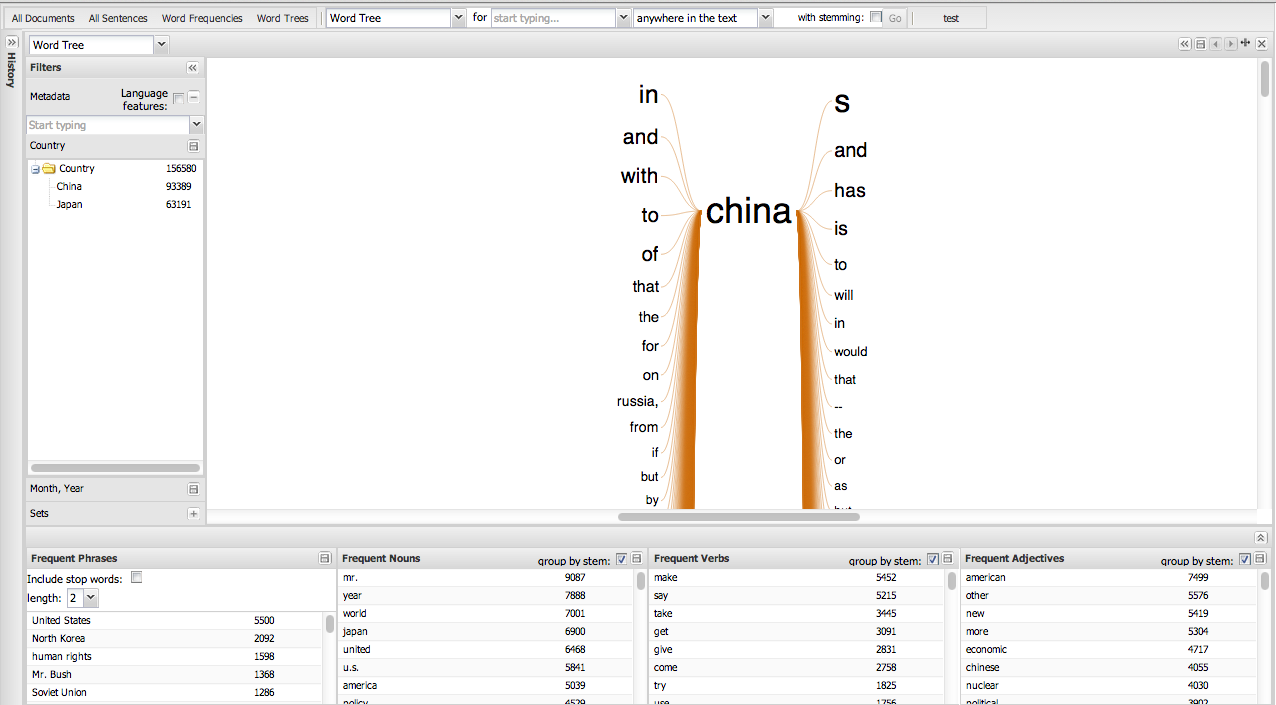
\includegraphics[width=0.5\textwidth]{fig/intro/01.png}
        }%
        \\
        \subfigure[A breakdown of the components of the user interface  \label{fig:intro02}]{%
	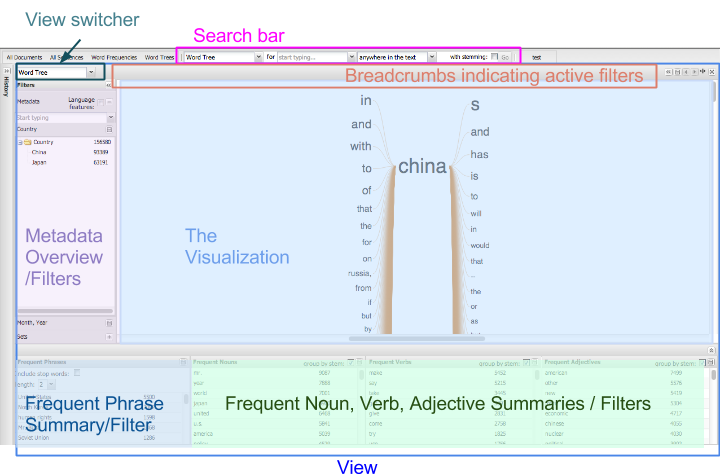
\includegraphics[width=0.5\textwidth]{fig/intro/02.png}
        }%
%
    \end{center}
    \caption{%
       Views in WordSeer.
     }%
\end{figure}

\subsection{Slices}

The easiest way to make slices in WordSeer is by intersecting \emph{searches} and \emph{filters}.  A search restricts the collection to just the sentences matching the query, and a filter restricts it to just sentences matching a particular metadata value. 
\begin{figure}[ht!]
\begin{center}
	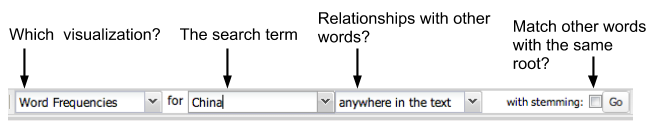
\includegraphics[width=0.5\textwidth]{fig/intro/03b.png}
\end{center}
    \caption{%
        Searching for sentences matching ``China''.\label{fig:intro03}
     }%
\end{figure}
One of C.F's first goals was to get a sense of the different ways China was discussed in the `80s, `90s and `00s. To do this, he assembled three slices, one for each decade, by starting with a \emph{search} for ``China'' (Figure \ref{fig:intro03})  and then filtering the `Year' category to range over each ten-year period (Figure \ref{fig:intro04a}).  WordSeer does not require metadata to be numerical ranges, it can also work with categorical values. If he had wanted to, C.F. could have filtered these results to just editorials whose main topic tag was China or Japan, using the controls shown in Figure \ref{fig:intro04b}. 

WordSeer's overviews showed clear differences between the decades. In particular, the increasing  frequencies of growth-related verbs contributed to a sense of China's rise, as shown by the frequencies per decade below:
\begin{itemize}
\item ``grow, growing'':  294, 232, 421
\item ``rise, rising'': 101, 134, 249
\item ``develop, developing'': 274, 404, 476
\end{itemize}

\subsection{Associated Slices}

 In the database, each sentence is indexed according to the following linguistic phenomena:
\begin{itemize}
  \item Each word in the sentence, and its part of speech (noun, verb, adjective, etc.),
  \item Each consecutive two-, three-, and four-word sequence in the sentence,
  \item Each grammatical relationship in the sentence. 
  \end{itemize}  
 By traversing these indexes, we can compute the associations for a slice. From a slice, we can query for all the words, phrases, or grammatical relations in the sentences in that slice, and from there, to all the other sentences that contain each particular item.  

 Grammatical relationships are identified using the Stanford dependency parser\cite{klein_accurate_2003} which extracts many kinds of relationships; some of the more easily understood ones include \emph{noun compound}, where two nouns come together to signify a new concept, \emph{adjective modifier} where an adjective describes another word, and \emph{direct subject} in which a word is the agent of a verb. 

Each view automatically presents the most common nouns, verbs, adjectives, and phrases (Figure \ref{fig:intro06}),  along with their counts (providing a query preview \cite{donn_query_1996} in a panel at the bottom.

\begin{figure}[h!]
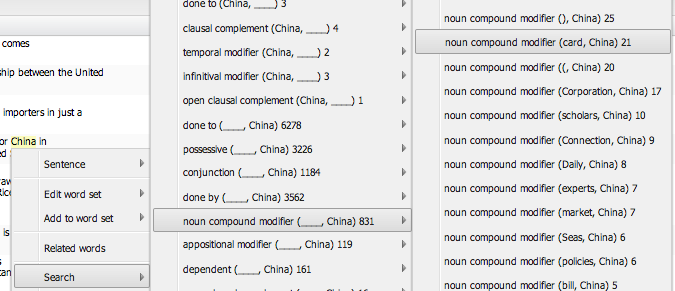
\includegraphics[width=0.5\textwidth]{fig/chris/01.png}
\caption{The word menu for `China'.   After selecting \emph{China > Search > noun compound modifier}, the noun-compound relationship ``China card'' stood out to C.F. \label{fig:chris01}}
\end{figure}

Individual words are jumping-off points. They can be acted upon wherever they appear via the Word Menu (Figure \ref{fig:chris01}) which enables  \emph{lateral movement}.  Any time a user sees a word, they can follow up on it by examining the grammatical relations in which it occurs, seeing related words,  and creating visualizations of the slice of sentences that contains the word, as well as the slices containing various relationships to other words.

The related words option in the Word Menu shows the nouns, verbs, and adjectives that co-occur most frequently with the clicked-on word. For example, if we click on `Japan' and open up the related words (Figure \ref{fig:intro09}) the pop-up shows the words that co-occur most frequently with `Japan' in this collection. Each of these related words can be clicked in turn, opening up a new Word Menu. These menus have the additional option to `See co-occurences', as shown in the new Word Menu for `exports'.  Selecting that option opens up a new view showing just those sentences in which the two words appear together  (in this case, `Japan' and `exports').  

The word menu reduces friction in both discovery and search. It only takes one menu click to discover that `exports' occurs frequently with `Japan', and only one more to see all the sentences in which `Japan' and `exports' are mentioned together.  


\subsection{Custom Slices with Sets}

Searches and filters are useful, but cannot always express  specific analysis goals. WordSeer therefore allows users to construct custom slices through Word-, Sentence-, and Document Sets. These custom slices behave like any other slices, which means that they can be summarized in views,  analyzed, filtered and searched. But they are more powerful that other slices because they also behave like metadata, transforming them into \emph{categorical filters}.

Word Sets are well-illustrated by an example from Case Study 1.  One concept of interest in this study was ``growth''. The scholar wished to confirm his intuitions about China's rise by checking whether  growth-related words became more frequent over time in editorials about China. First, he created a new Word Set and typed in some growth-related words ``growing, develop, developing, grow, rise, rising" (Figure \ref{fig:intro10a-word-sets}). The result was a Word Set representing a new slice of sentences, those containing at least one of those words. 


After the Word Set is created, the entire user interface responds to its presence. The search box now shows a drop-down option for the set  (Figure \ref{fig:intro10b-word-sets}).  The Word Menu shows the option to add a new words (Figure \ref{fig:intro10c-word-sets}) and the metadata overviews (Figure \ref{fig:intro10d-word-sets}), previously restricted to pre-defined categories,  now show this new ``category'', and allows C.F. to filter based on it.   

\begin{figure}[ht!]
\begin{center}
	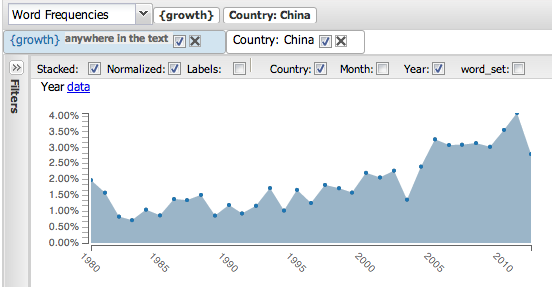
\includegraphics[width=0.5\textwidth]{fig/chris/04a.png}
\end{center}
    \caption{%
	The \code{\{growth\}} Word Set used as a Word Frequencies query.\label{fig:chris04a}
     }%
\end{figure}

To verify that China was indeed described as rising, C.F. selected the  \code{\{growth\}} Word Set as his search query, and opened a Word Frequencies view with the  \code{ country = China} filter. The resulting visualization is Figure \ref{fig:chris04a}, which shows almost a doubling of the frequency of these words in editorials about China over the 30-year period from 1980 to 2012. Satisfied that WordSeer was capable of reproducing this widely accepted fact, he was able to move on to deeper questions.

For sentences and documents, the idea is the same.  Users can hand-pick collections of sentences from the reading view, and from search results view, or collections of documents from the document search results view.  Once created, all these sets can be overviewed and analyzed like any other slice, and additionally used as filters.

\bibliographystyle{abbrv}
\bibliography{old_cikm} 

\newpage
\appendix
\begin{figure}[h!]
\begin{center}
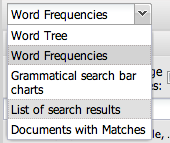
\includegraphics[width=0.2\textwidth]{fig/chris/03.png}
\end{center}
\caption{ The view-switcher drop-down menu.\label{fig:chris03}}
\end{figure}


\begin{figure}[ht!]
\begin{center}
%
        \subfigure[C.F. used the date-range overview to select the slice ``all sentences from the 1990's matching \emph{China}'']{%
            \label{fig:intro04a}
	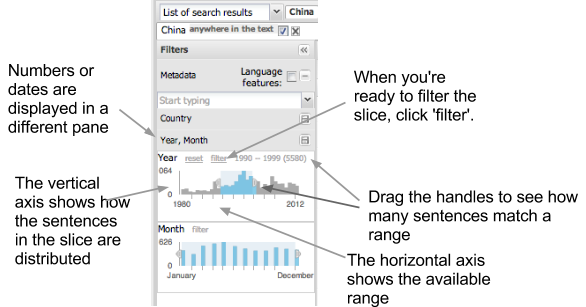
\includegraphics[width=0.5\textwidth]{fig/intro/04b.png}
        }%
        \\
         \subfigure[Clicking on a value will filter the slice to match. For example, clicking on `China' would create the slice  ``all sentences containing \emph{China} from editorials about China''.]{%
            \label{fig:intro04b}
	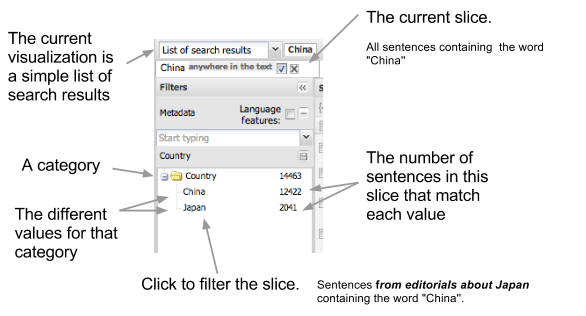
\includegraphics[width=0.5\textwidth]{fig/intro/04a.png}
        }%
%
    \end{center}
    \caption{%
     Both types of overviews double as filters \label{fig:intro04}.
     }%
\end{figure}

\begin{figure}[ht!]
\begin{center}
	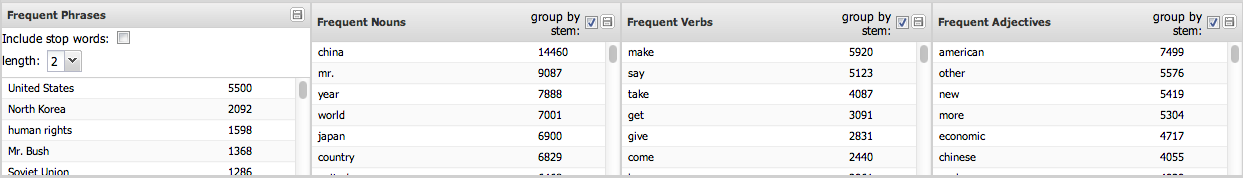
\includegraphics[width=0.5\textwidth]{fig/intro/06.png}
\end{center}
    \caption{%
       The most frequent phrases, nouns, verbs, and adjectives in the \emph{New York Times} editorials for Case Study 1.  \label{fig:intro06}
     }%
\end{figure}

\begin{figure}[ht!]
\begin{center}
	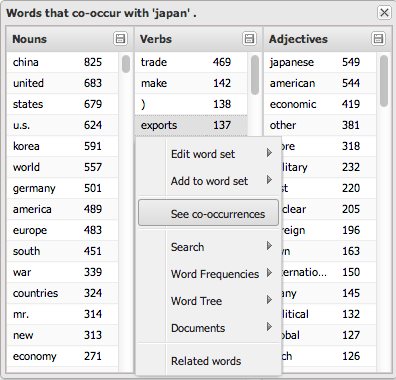
\includegraphics[width=0.3\textwidth]{fig/intro/09.png}
\end{center}
    \caption{%
 		The words that co-occur most frequently with `Japan'. Clicking on any of these words opens up a Word Menu, this time with the option to see the sentences containing the co-occurrence.
	\label{fig:intro09}}%
\end{figure}

\begin{figure}[ht!]
\begin{center}
%
        \subfigure[Creating a ``growth'' word set with 6 words in it. \label{fig:intro10a-word-sets}]{%
	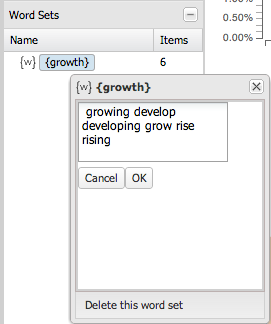
\includegraphics[width=0.2\textwidth]{fig/intro/10a-word-sets.png}
        }%
        \\
        \subfigure[The set now appears in the drop-down menu in the search box. \label{fig:intro10b-word-sets}]{%
	
\includegraphics[width=0.5\textwidth]{fig/intro/10b-word-sets.png}
        }%
         \\
        \subfigure[The set also appears in the word menu  \label{fig:intro10c-word-sets}]{%
	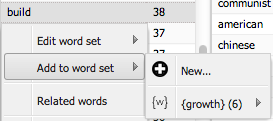
\includegraphics[width=0.2\textwidth]{fig/intro/10c-word-sets.png}
        }%
        \quad
        \subfigure[ The set also appears in the metadata overview   \label{fig:intro10d-word-sets}]{%
	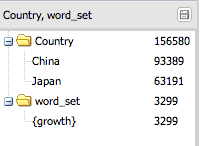
\includegraphics[width=0.2\textwidth]{fig/intro/10d-word-sets.png}
        }%
%
    \end{center}
    \caption{%
       Word Sets in WordSeer. \label{fig:intro10-word-sets}
     }%
\end{figure}


\end{document}


